\documentclass[../main.tex]{subfiles}	

\begin{document}

\chapter{Domain Adaptation}
\label{ch:domain_adaptation}

In the last chapter of this thesis work, we want to address another important field of machine learning, with which can complete our previous discussion about condition monitoring, i.e. domain adaptation. Domain adaptation is an area of \textit{transfer learning}, dedicated to the study of those scenarios in which we aim at generalizing an high performance learner on a target domain via utilizing the knowledge distilled on a source domain which has a different but related data distribution.\\
The starting point of this last analysis is the observation that those simulations, constructed to collect the data we have used to approach the healthy-faulty classification problems in the last chapter, have some inherent dissimilarities with the real-world situations. We expect, in fact, to have much less faulty conditions in practice, and so the datasets we have used up to now were not properly balanced, with fault signals being overrepresented. This is the main reason for which we need a working strategy suitable to extend, to \textit{transfer}, the knowledge that our models learned from simulated data to a "target" set, constituted by more "realistic", often unlabeled, samples. And this strategy can be found exactly in this area known as domain adaptation. \\
In particular, we are going to deepen a recent transfer learning strategy known as \textbf{Wasserstein Distance Guided Representation Learning} (WDGRL) \cite{shen2018wasserstein}, that we believe it could be the starting point for future studies in domain adaptation for complex-valued deep learning. This approach is, in fact, based on the optimization problem of a measure that can we can extend, without ambiguity, also in the complex domain, i.e. the Wasserstein Distance. \\
We also maid several tests considering a possible alternative to WDGRL, also this with a trivial extent in the complex domain, i.e. \textbf{Adversarial Domain Adaptation} \cite{adversarial_domain_adaptation, ajakan2015domainadversarial, ganin2016domainadversarial}: the fundamental concepts behind DANN (deep adversarial neural networks) 
We didn't manage, however, to obtain any consisted and/or stable results using this methodology, and so we decided only to cite it.\\
We believe that the nice results (at least qualitatively) we have achieved, could be a nice starting point for future, more detailed works, as apparently, no domain adaptation approach has been proposed for complex-valued inputs yet.

\section{Wasserstein Distance Guided Representation Learning}

One of the most common strategies for domain adaptation is to learn domain-invariant feature representations that have to be also discriminative in
prediction. To do this, usually domain adaptation frameworks are based on both a learning approach to measure and reduce the domain discrepancy, as well as a discriminator for classification. The 

\begin{figure}[!ht]
	\centering
	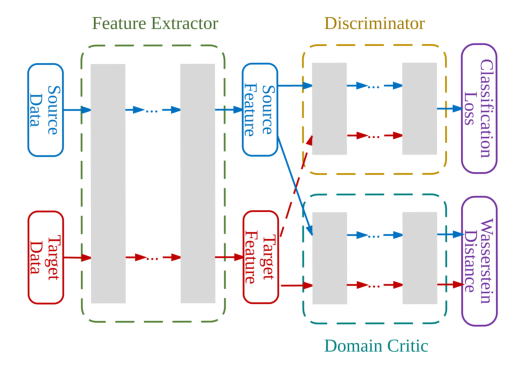
\includegraphics{pictures/wdgrl_scheme}
	\caption{Network scheme of Wassersten Distance Guided Representation Learning applied to a classification task.}
	\label{fig:wdgrl_scheme}
\end{figure}



\section{Domain Adaptation of Bonfiglioli Data}

In section \ref{sec:mendeley_analysis}, with the objective of showing the generalization properties of complex-valued models, we divided the Mendeley dataset into smaller subsets, according to their specific time-varying speed conditions, and we trained the model over only of those. In that case we were able to guarantee nice accuracies in almost all the combinations of training-test sets, proving that 
The fact is that, in the above case, the experimental setup, except for the rotational dynamics, were identical among train and test subsets. But for the data provided by Bonfiglioli, the situation is much more complicated: those datasets differ not only by the fault simulated, but also by the engine that is begin tested. We will see that both real and complex-valued models underperform, sometimes becomes even completely unable, to distinguish among signals originated by different motors.\\
In order to properly simulate a real-world situation, in which engine's faults are quite rare and most of the signals measured are healthy, we proceeded as follow:
\begin{itemize}
	\item the trials in the source were split into a $75\%-25\%$ train-test sets;
	\item for the trials in the target, the faulty samples were all put in the target-test set, while the healthy samples were split among target-train and target-test sets with the same percentage as before; in this way the target-train set is completely constituted by healthy samples (even if, officially, from the point of view of the models, those samples are unlabeled). 
\end{itemize}
There are two cases, among the Bonfiglioli datasets, that we found interesting to consider for domain adaptation:
\begin{itemize}
	\item \textit{Trials 4 and 5 versus trial 6}: in this configuration, the source set contains both the information about the mechanical engine (trial 4) and about the kind of fault (trial 5) of the target distribution (trial 11) and so we believe it constitutes the ideal case for testing domain adaptation.
	\item \textit{Trial 10\_1 vs trial 10\_4}: this is a particular case, since the both datasets have been collected over the same setup, with the same rotational gearmotor and same kind of fault; the only difference, in this case, is that the two experimental axis, healthy and faulty, have been inverted (this was done in order to ensure that our machine learning models were not trained to "learn the axis" but to recognize the fault).
\end{itemize}
In both cases, in fact, the classifiers developed, even guaranteeing nice performances over the source distributions, were not able alone to generalize properly over signals belonging to the target distribution, regardless of the similarity of the two.\\
There were also cases in which, even implementing domain adaptation, we weren't able to make the model converge, sign that probably the two distributions are too different among each other. This is the case of \textit{trial 5 vs trial 11}: the two datasets share the same kind of fault simulated, but contains signals collected from different engines, and apparently this constituted a huge obstacle to generalization (also with conventional real-valued approaches).\\
Regarding the models that we have used in our analysis, we can say that they have essentially the same structure of the ones built in the classification tasks (figure \ref{}). The feature extractor is constituted by the first part of the complex-valued model (basically the three convolutional layers) up to the flattening step, while the discriminator and the domain critic are simple multi-layer perceptrons with structure $Linear(32)\to Linear(8)\to Linear(n)$, with $n$ being the number of classes for the first, and $n=1$ for the latter.
 
\subsection*{Trials 4 and 5 versus trial 6}

In this first attempt we consider, as source set, the union of trials 4 (BN90, unbalance) and 5 (BMD118, bearing) while trial 6 (BN90, bearing) will be our target set, split into target-train and target-test as explained above. We have already said that this combination of dataset can, in theory, provide some results, since the source sets contain the necessary information to make our models performing well also on the target set. Let's start showing how limited are the generalization performances of our complex-valued architecture and its real counterpart. For simplicity, we first considered the problem as a binary classification task, with only labels "healthy" and "faulty" and not caring about the two different types of fault. Then, training the networks over the source-train set, in table \ref{tab:bonfiglioli_binary_generalization_456} we report the accuracies obtained after the convergence.
\begin{table}[!ht]
	\centering
	\begin{minipage}{.45\linewidth}
		\begin{tabular}{c c}
			\textbf{Source test} & \textbf{Target}\\
			\midrule
			99.94\% & 65.28\% \\			
		\end{tabular}
	\end{minipage}
	\begin{minipage}{.45\linewidth}
		\begin{tabular}{c c}
			\textbf{Source test} & \textbf{Target}\\
			\midrule
			99.94\% & 59.59\% \\			
		\end{tabular}
	\end{minipage}
	\caption{Generalization performances, in term of accuracy, of real (left) and complex-valued (right) convolutional neural networks in the binary domain adaptation problem 4-5 vs 6.}
	\label{tab:bonfiglioli_binary_generalization_456}
\end{table}
This time we see the real-valued model providing the higher accuracy: we noticed, however, that, in the training loop, the crossentropy decreased a lot, much more than in the complex case. Looking also at the results achieved in previous chapters, we believe that this is just sign of higher overfitting and instability. In table \ref{tab:bonfiglioli_multiclass_generalization_456}, in fact, we put the results of the same problem, but this time keeping the two faults distinct, such that the models will have to distinguish among 3 classes.
\begin{table}[!ht]
	\centering
	\begin{minipage}{.45\linewidth}
		\begin{tabular}{c c}
			\textbf{Source test} & \textbf{Target}\\
			\midrule
			99.94\% & 31.28\% \\			
		\end{tabular}
	\end{minipage}
	\begin{minipage}{.45\linewidth}
		\begin{tabular}{c c}
			\textbf{Source test} & \textbf{Target}\\
			\midrule
			99.84\% & 35.16\% \\			
		\end{tabular}
	\end{minipage}
	\caption{Generalization performances, in term of accuracy, of real (left) and complex-valued (right) convolutional neural networks in the multiclass domain adaptation problem 4-5 vs 6.}
	\label{tab:bonfiglioli_multiclass_generalization_456}
\end{table}
The performances decreases drastically, but this time, it is the complex network that wins the competition. This can also be interpreted as the nth sign that those models are more robust in case of "critical" situations.\\



\subsection*{Trial 10\_1 vs trial 10\_4}

We have already presented the peculiarity of this combination of datasets, characterized by the same mechanical components, but with the faults simulated in different axis. Apparently, this is enough to change completely the nature of the signals measured. Repeating the same preliminaries tests as for the other configuration (table \ref{tab:bonfiglioli_generalization_101_104}), this time the accuracy values are higher, and we notice a clear advantage of the complex model ($+10\%$).
\begin{table}[!ht]
	\centering
	\begin{minipage}{.45\linewidth}
		\begin{tabular}{c c}
			\textbf{Source test} & \textbf{Target}\\
			\midrule
			99.64\% & 76.13\% \\			
		\end{tabular}
	\end{minipage}
	\begin{minipage}{.45\linewidth}
		\begin{tabular}{c c}
			\textbf{Source test} & \textbf{Target}\\
			\midrule
			100.00\% & 66.46\% \\			
		\end{tabular}
	\end{minipage}
	\caption{Generalization performances, in term of accuracy, of real (left) and complex-valued (right) convolutional neural networks in the multiclass domain adaptation problem 4-5 vs 6.}
	\label{tab:bonfiglioli_generalization_101_104}
\end{table}




\end{document}